% METODOLOGIA------------------------------------------------------------------

\chapter{METODOLOGIA}
\label{chap:metodologia}

Para uma melhor organização, a efetivação do trabalho é composta por duas partes, onde a primeira é a coleta de dados e, a segunda, o desenvolvimento da aplicação. 
Na segunda parte da execução do trabalho, será o desenvolvimento do algoritmo de reconstrução, que consistirá em quatro etapas, no qual, para cada etapa é desenvolvido uma rotina. 
Primeiro os dados serão preparados, em seguida serão refinados e filtrados, por fim, renderizados.
O produto final do processamento, será uma superfície tridimensional.
Cada parte está segmentada em etapas, no qual cada etapa é um processo a ser executado. Por conseguinte, a organização da metodologia apresenta os itens:

\begin{itemize}
    \addtolength{\itemindent}{2em}
    
    \item Coleta de dados
    \begin{itemize}
        \addtolength{\itemindent}{2em}
        
        \item Dados em simulação
        \item Dados \textit{in loco}
    \end{itemize}
    
    \item Desenvolvimento
    \begin{itemize}
        \addtolength{\itemindent}{2em}
        
        \item Pré-processamento
        \item Filtragem
        \item Reconstrução
        \item Comparação
    \end{itemize}
\end{itemize}
\hspace{1em}

A Figura \ref{fig:etapas} mostra as etapas do desenvolvimento da aplicação. Primeiramente, os dados são inseridos através de um \textit{dataset}, em verde são representados as etapas do pré-processamento, em amarelo são representados os processos de filtragem, o processo de reconstrução é representado em marrom, e por fim, a superfície é gerada.
A etapa de comparação requer duas superfícies na entrada do processo, para gerar a superfície resultante.


\begin{figure}[H]
    \centering
    \caption{Etapas do processo de desenvolvimento da aplicação.}
    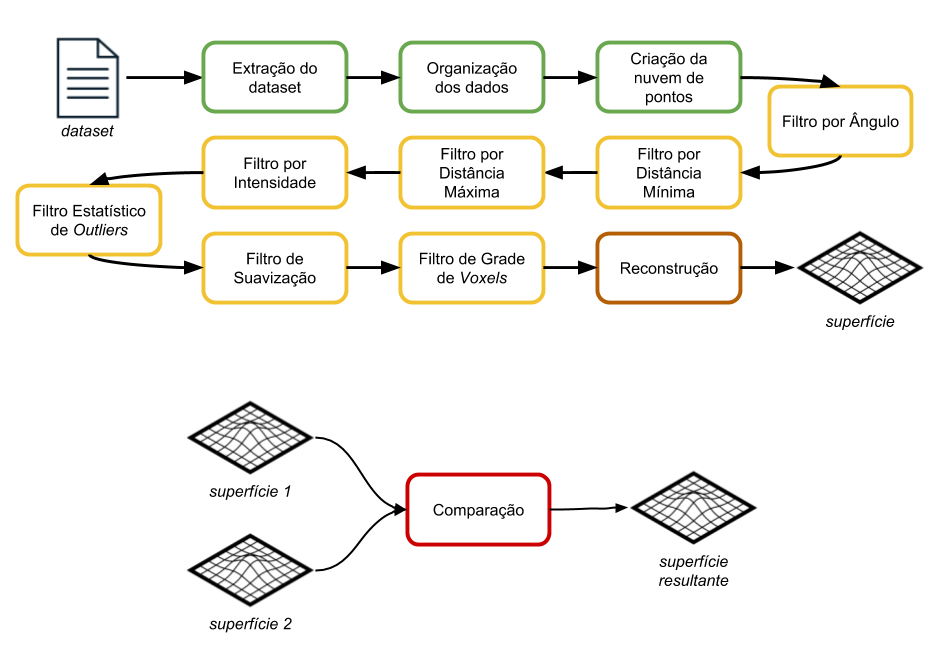
\includegraphics[scale=0.4]{dados/figuras/etapas.png}
    \label{fig:etapas}
\end{figure}

\section{Coleta de dados}
\label{sec:coleta_dados}

A coleta de dados foi realizada de duas formas: em simulação virtual e \textit{in loco}. 
A coleta em simulação virtual facilita a obtenção de dados, por não haver a necessidade de possuir um sensor ou robô e por dispensar planejamento logístico que uma saída de campo requer. 
Contudo, é importante fazer a coleta \textit{in loco}, pois possibilita realizar a comparação do desempenho do algoritmo e, além disso, as informações obtidas serão mais próximo do mundo real quanto às coletadas em simulação.

\subsection{Simulação virtual}
\label{sec:simulation}

A obtenção de dados por simulação virtual contará com o auxílio de \textit{softwares} e ferramentas. 
O \textit{software} Gazebo será o responsável por simular o ambiente virtual, enquanto que o ROS será responsável por executar o modelo do veículo ROV e o simulador do sonar MSIS.
O veículo ROV utilizado, chamado RexROV (Figura \ref{fig:rexrov}), foi desenvolvido pelos autores \cite{manhaes2016uuv} e está incluso no pacote \textit{UUV Simulator}.
O ambiente de simulação, apresentado na Figura \ref{fig:environment}, representa o fundo de um corpo d'água.
Assim como o robô, o ambiente de simulação também está disponível no pacote \textit{UUV Simulator}.

\begin{figure}[H]
    \centering
    \caption{Veículo e ambiente utilizado na simulação virtual.}
    \label{fig:simulation}
    \begin{subfigure}[t]{0.4\textwidth}
        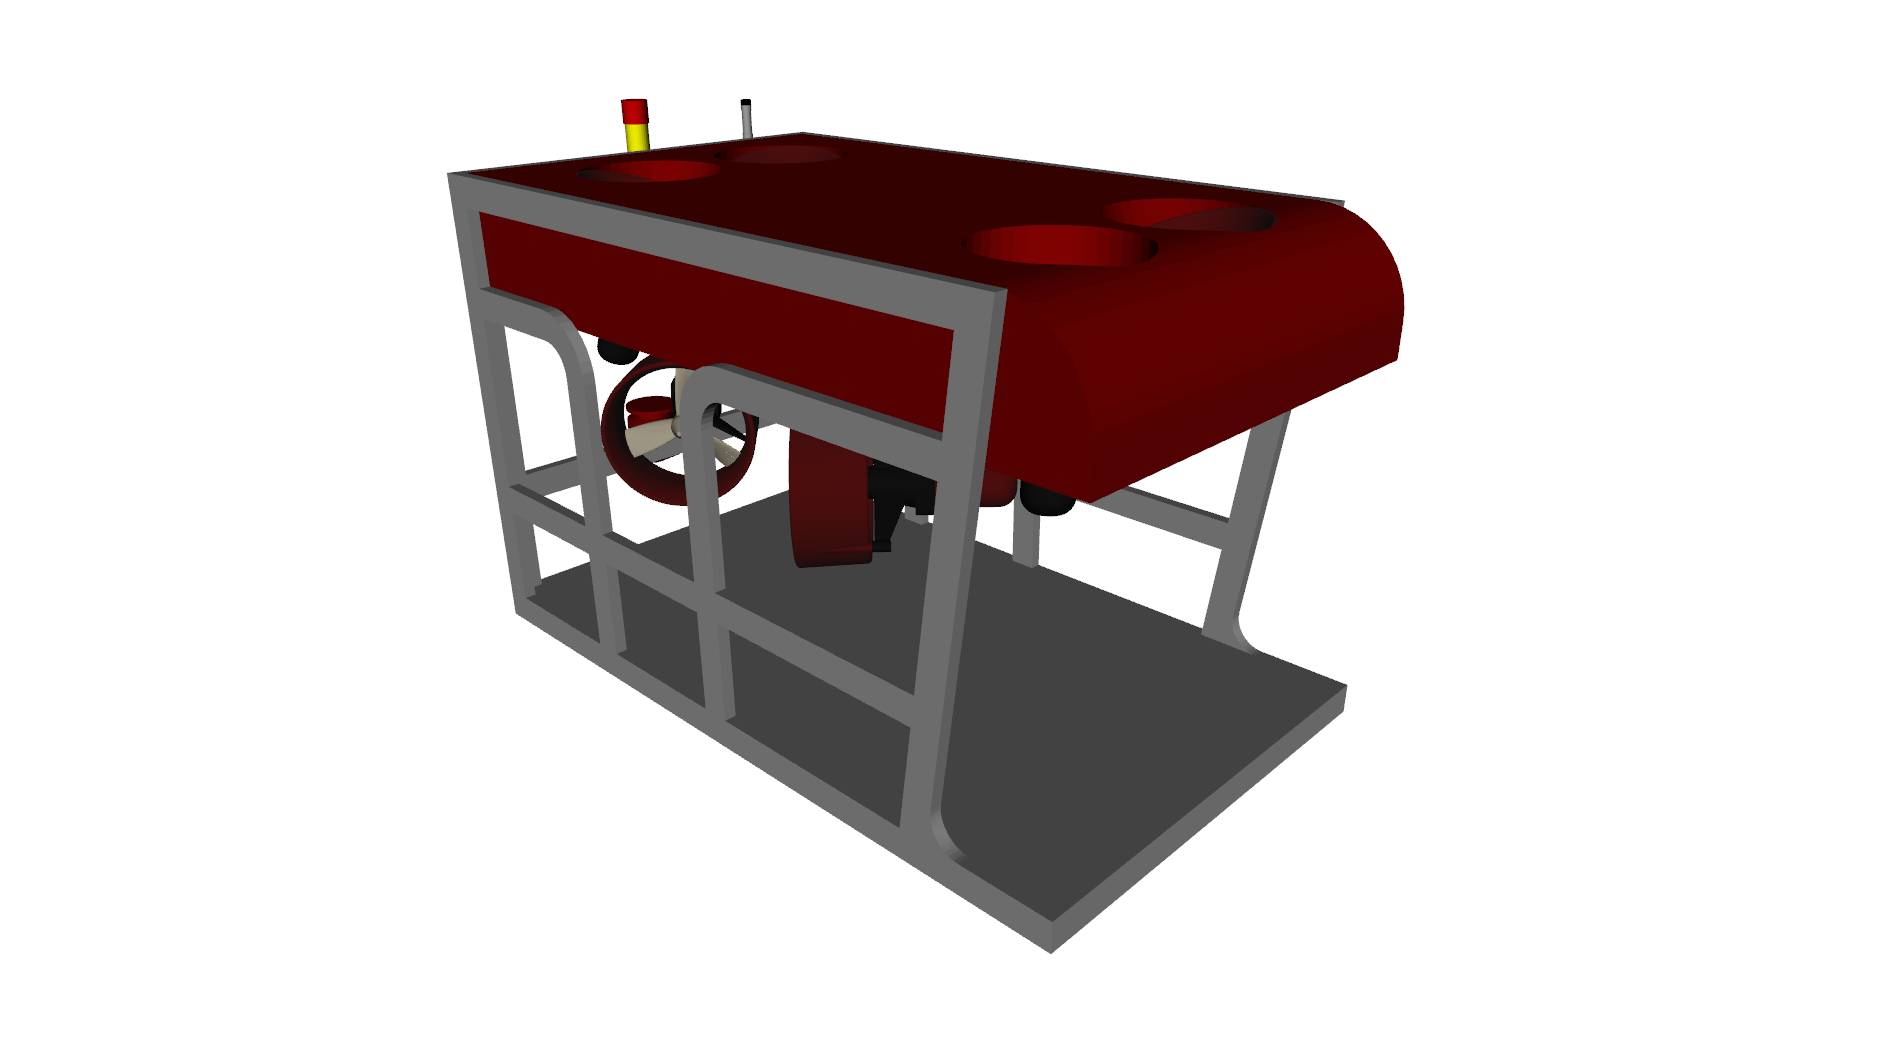
\includegraphics[width=\textwidth]{dados/figuras/rexrov.png}
        \caption{Veículo RexROV.}
        \label{fig:rexrov}
    \end{subfigure}
    \hspace{1em}
    \begin{subfigure}[t]{0.55\textwidth}
        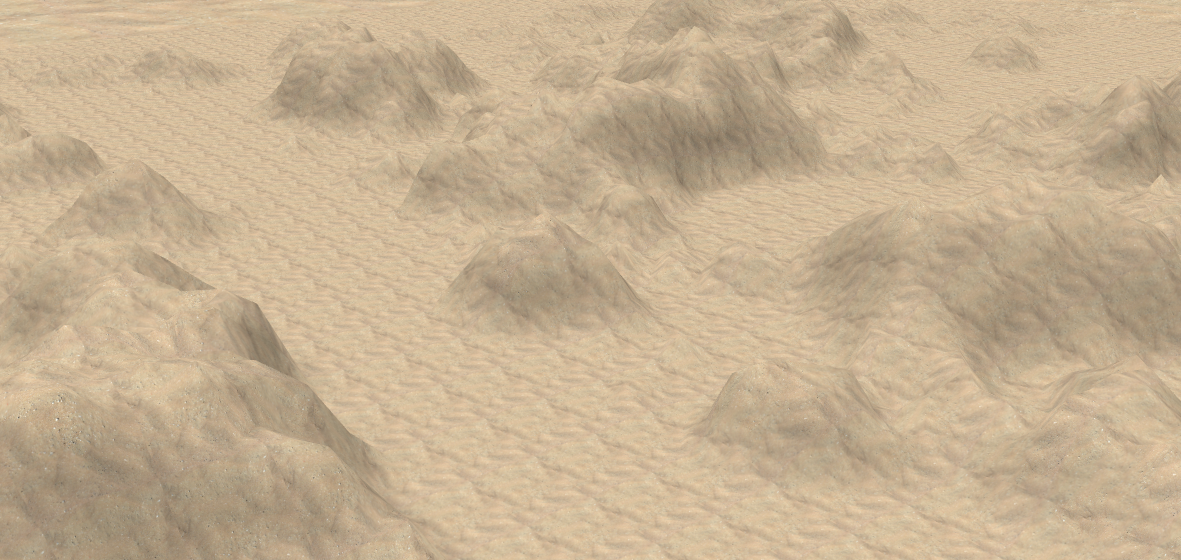
\includegraphics[width=\textwidth]{dados/figuras/environment.png}
        \caption{Ambiente em simulação.}
        \label{fig:environment}
    \end{subfigure}
\end{figure}

Em simulação, as unidades utilizadas para o comprimento não estão definidas em metros, por esse motivo qualquer comprimento descrito no ambiente de simulação será na sigla \textit{uc} (unidades de comprimento).
No ambiente, como mostra a Figura \ref{fig:scenaries}, foi acrescentado obstáculos para montar diferentes tipos de cenários.
No cenário \textbf{a} e \textbf{b} foram acrescentadas a mesma parede, a diferença está na posição no segundo cenário está 5\textit{uc} mais distante em relação ao primeiro cenário.

\begin{figure}[H]
    \centering
    \caption{Cenários criados para realizar o experimento.}
    \label{fig:scenaries}
    \begin{subfigure}[t]{0.328\textwidth}
        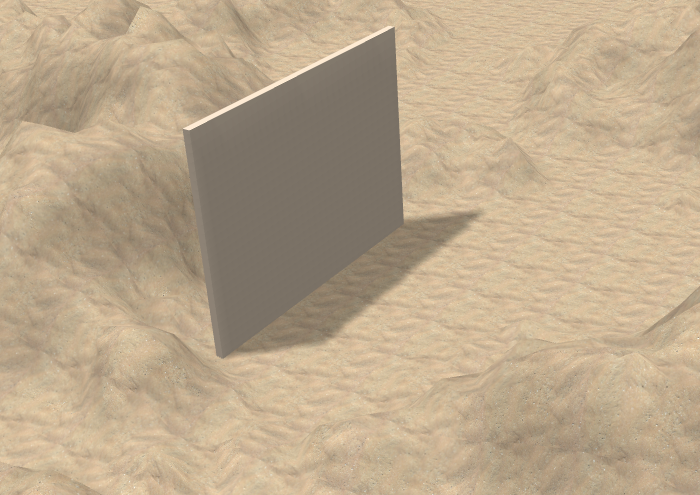
\includegraphics[width=\textwidth]{dados/figuras/scene3.png}
        \caption{}
        \label{fig:scene2}
    \end{subfigure}
    \begin{subfigure}[t]{0.328\textwidth}
        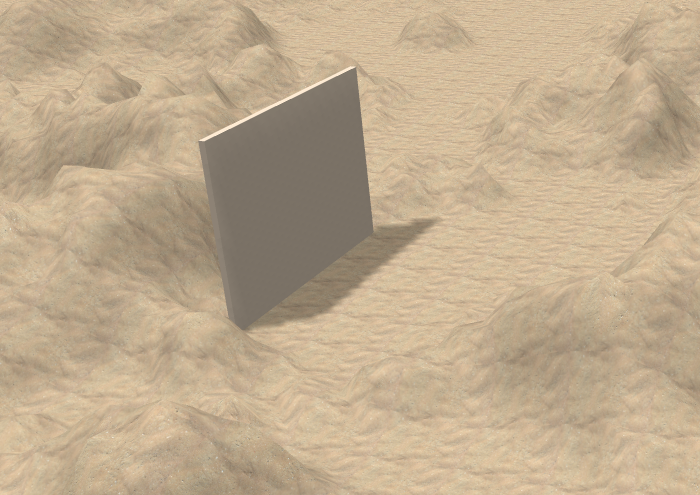
\includegraphics[width=\textwidth]{dados/figuras/scene2.png}
        \caption{}
        \label{fig:scene1}
    \end{subfigure}
    \begin{subfigure}[t]{0.328\textwidth}
        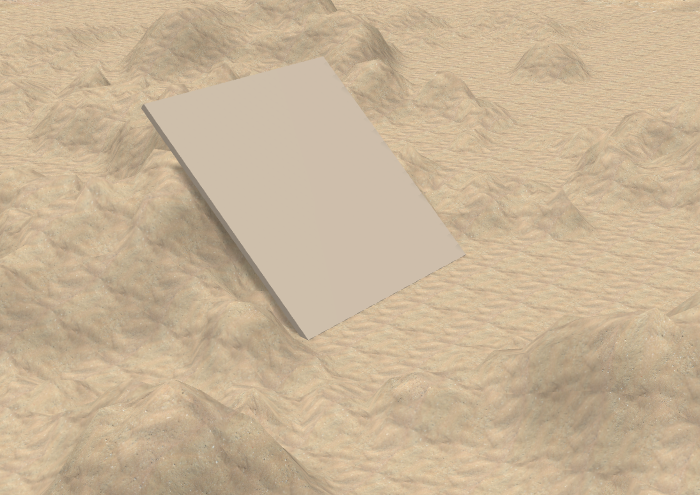
\includegraphics[width=\textwidth]{dados/figuras/scene4.png}
        \caption{}
        \label{fig:scene3}
    \end{subfigure}
\end{figure}

O cenário \textbf{c} foi construído a partir do cenário \textbf{a}, onde ocorre a inclinação em 45º da parede e alongamento da sua altura para manter a mesma da parede do cenário anterior.
A intenção é simular uma geleira em um estado inicial, representado pelo cenário \textbf{a}, e em um estado posterior após perder o volume inicial, representado pelos cenários \textbf{b} e \textbf{c}.
Portanto, a comparação de volume acontecerá em dois contextos: o primeiro contexto será chamado de \textbf{AB}, onde os cenários \textbf{a} e \textbf{b} estão envolvidos, no qual simula uma perda de volume, pois \textbf{a} está 5\textit{uc} à frente de \textbf{b}; o segundo contexto será chamado de \textbf{AC}, onde os cenários \textbf{a} e \textbf{c} estão envolvidos, no qual há uma perda menor de volume em relação ao primeiro contexto.
A Figura \ref{fig:dimensoes} exibe as dimensões das paredes utilizadas nas simulações.
O contexto é um cenário onde há dois modelos reconstruídos, que serve para fazer a comparação entre esses modelos.

\begin{figure}[H]
    \centering
    \caption{Dimensões das paredes.}
    \label{fig:dimensoes}
    \begin{subfigure}[t]{0.328\textwidth}
        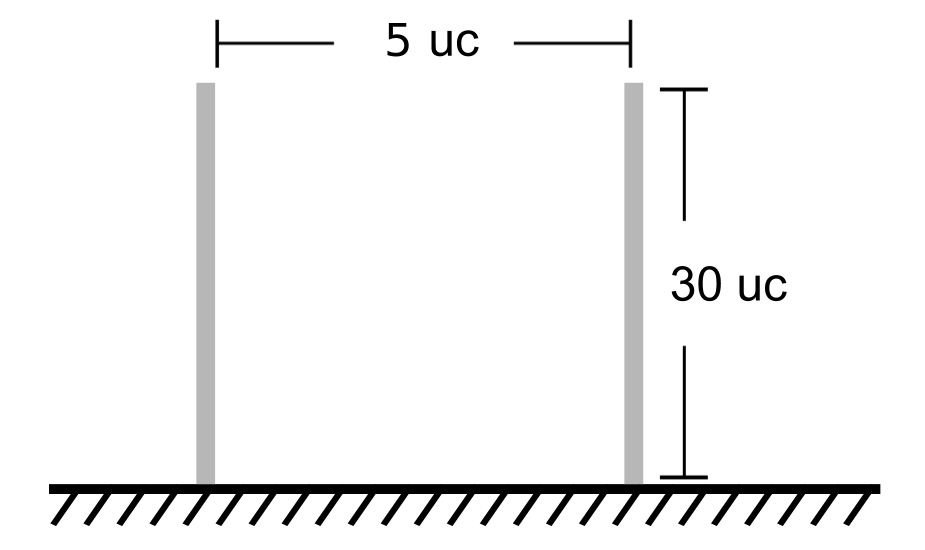
\includegraphics[width=\textwidth]{dados/figuras/dim_lateral_ab.png}
        \caption{Vista lateral entre \textbf{a} e \textbf{b}.}
        \label{fig:dim_lateral_ab}
    \end{subfigure}
    \begin{subfigure}[t]{0.328\textwidth}
        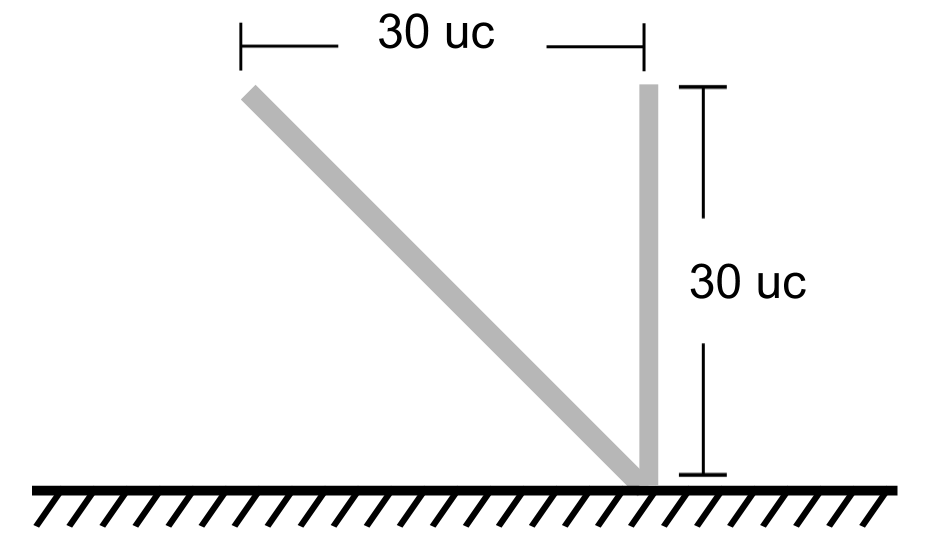
\includegraphics[width=\textwidth]{dados/figuras/dim_lateral_ac.png}
        \caption{Vista lateral entre \textbf{a} e \textbf{c}.}
        \label{fig:dim_lateral_ac}
    \end{subfigure}
    \begin{subfigure}[t]{0.328\textwidth}
        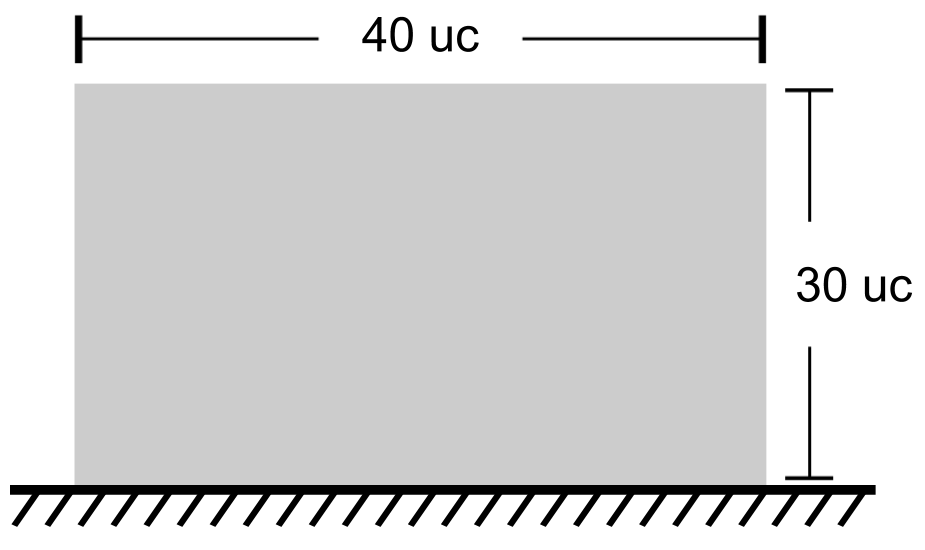
\includegraphics[width=\textwidth]{dados/figuras/dim_frontal.png}
        \caption{Vista frontal da parede.}
        \label{fig:dim_frontal}
    \end{subfigure}
\end{figure}

Em todos os \textit{datasets} criados, o ROV foi posicionado a uma distância de aproximadamente 25uc, iniciando a coleta na parte superior da superfície. 
Após o início, o sensor faz a leitura completa de uma imagem acústica, ou seja, o transdutor percorrer de 0º à  180º, gerando um \textit{beam} por grau.
Realizada a coleta de uma imagem acústica, o robô ativa os propulsores para se deslocar cerca de 0.7uc em direção ao solo. 
Após o deslocamento, o processo de leitura se repete até o veículo encostar no leito do corpo d'água.


\subsection{\textit{In loco}}
\label{sec:in_loco}

A aquisição de dados em campo foi realizada em uma piscina, como mostra a Figura \ref{fig:piscina}.
A piscina possui o formato de um retângulo no qual há dois lados maiores e dois lados menores, onde foi utilizado apenas um dos lados menores.

O ROV foi posicionado inicialmente à uma determinada distância da parede e próximo a superfície.
O sensor faz a leitura da parede, percorrendo 180º e na sequência se desloca alguns centímetros verticalmente em direção ao fundo.
Esse procedimento se repete até o robô encostar no fundo da piscina.
No primeiro experimento, o ROV foi posicionado a 1,5 metros de distância da parede da piscina, esse será o cenário D.
Após concluir a varredura, o procedimento é repetido, porém à uma distância de 3 metros, esse será o cenário E.
Ambos cenários vão compor o único contexto do experimento em campo.

\iffalse
O segundo experimento foi semelhante ao primeiro, porém foi realizado no outro lado, no qual possui uma escadaria, e as distâncias eram de 2,5 e 4 metros.
O cálculo de volume só haverá no primeiro experimento, pois no segundo, não há como saber o real valor do volume da escadaria.
\fi

\begin{figure}[H]
    \centering
    \caption{Piscina onde foram coletados os dados.}
    \label{fig:piscina}
    \begin{subfigure}[t]{0.25\textwidth}
        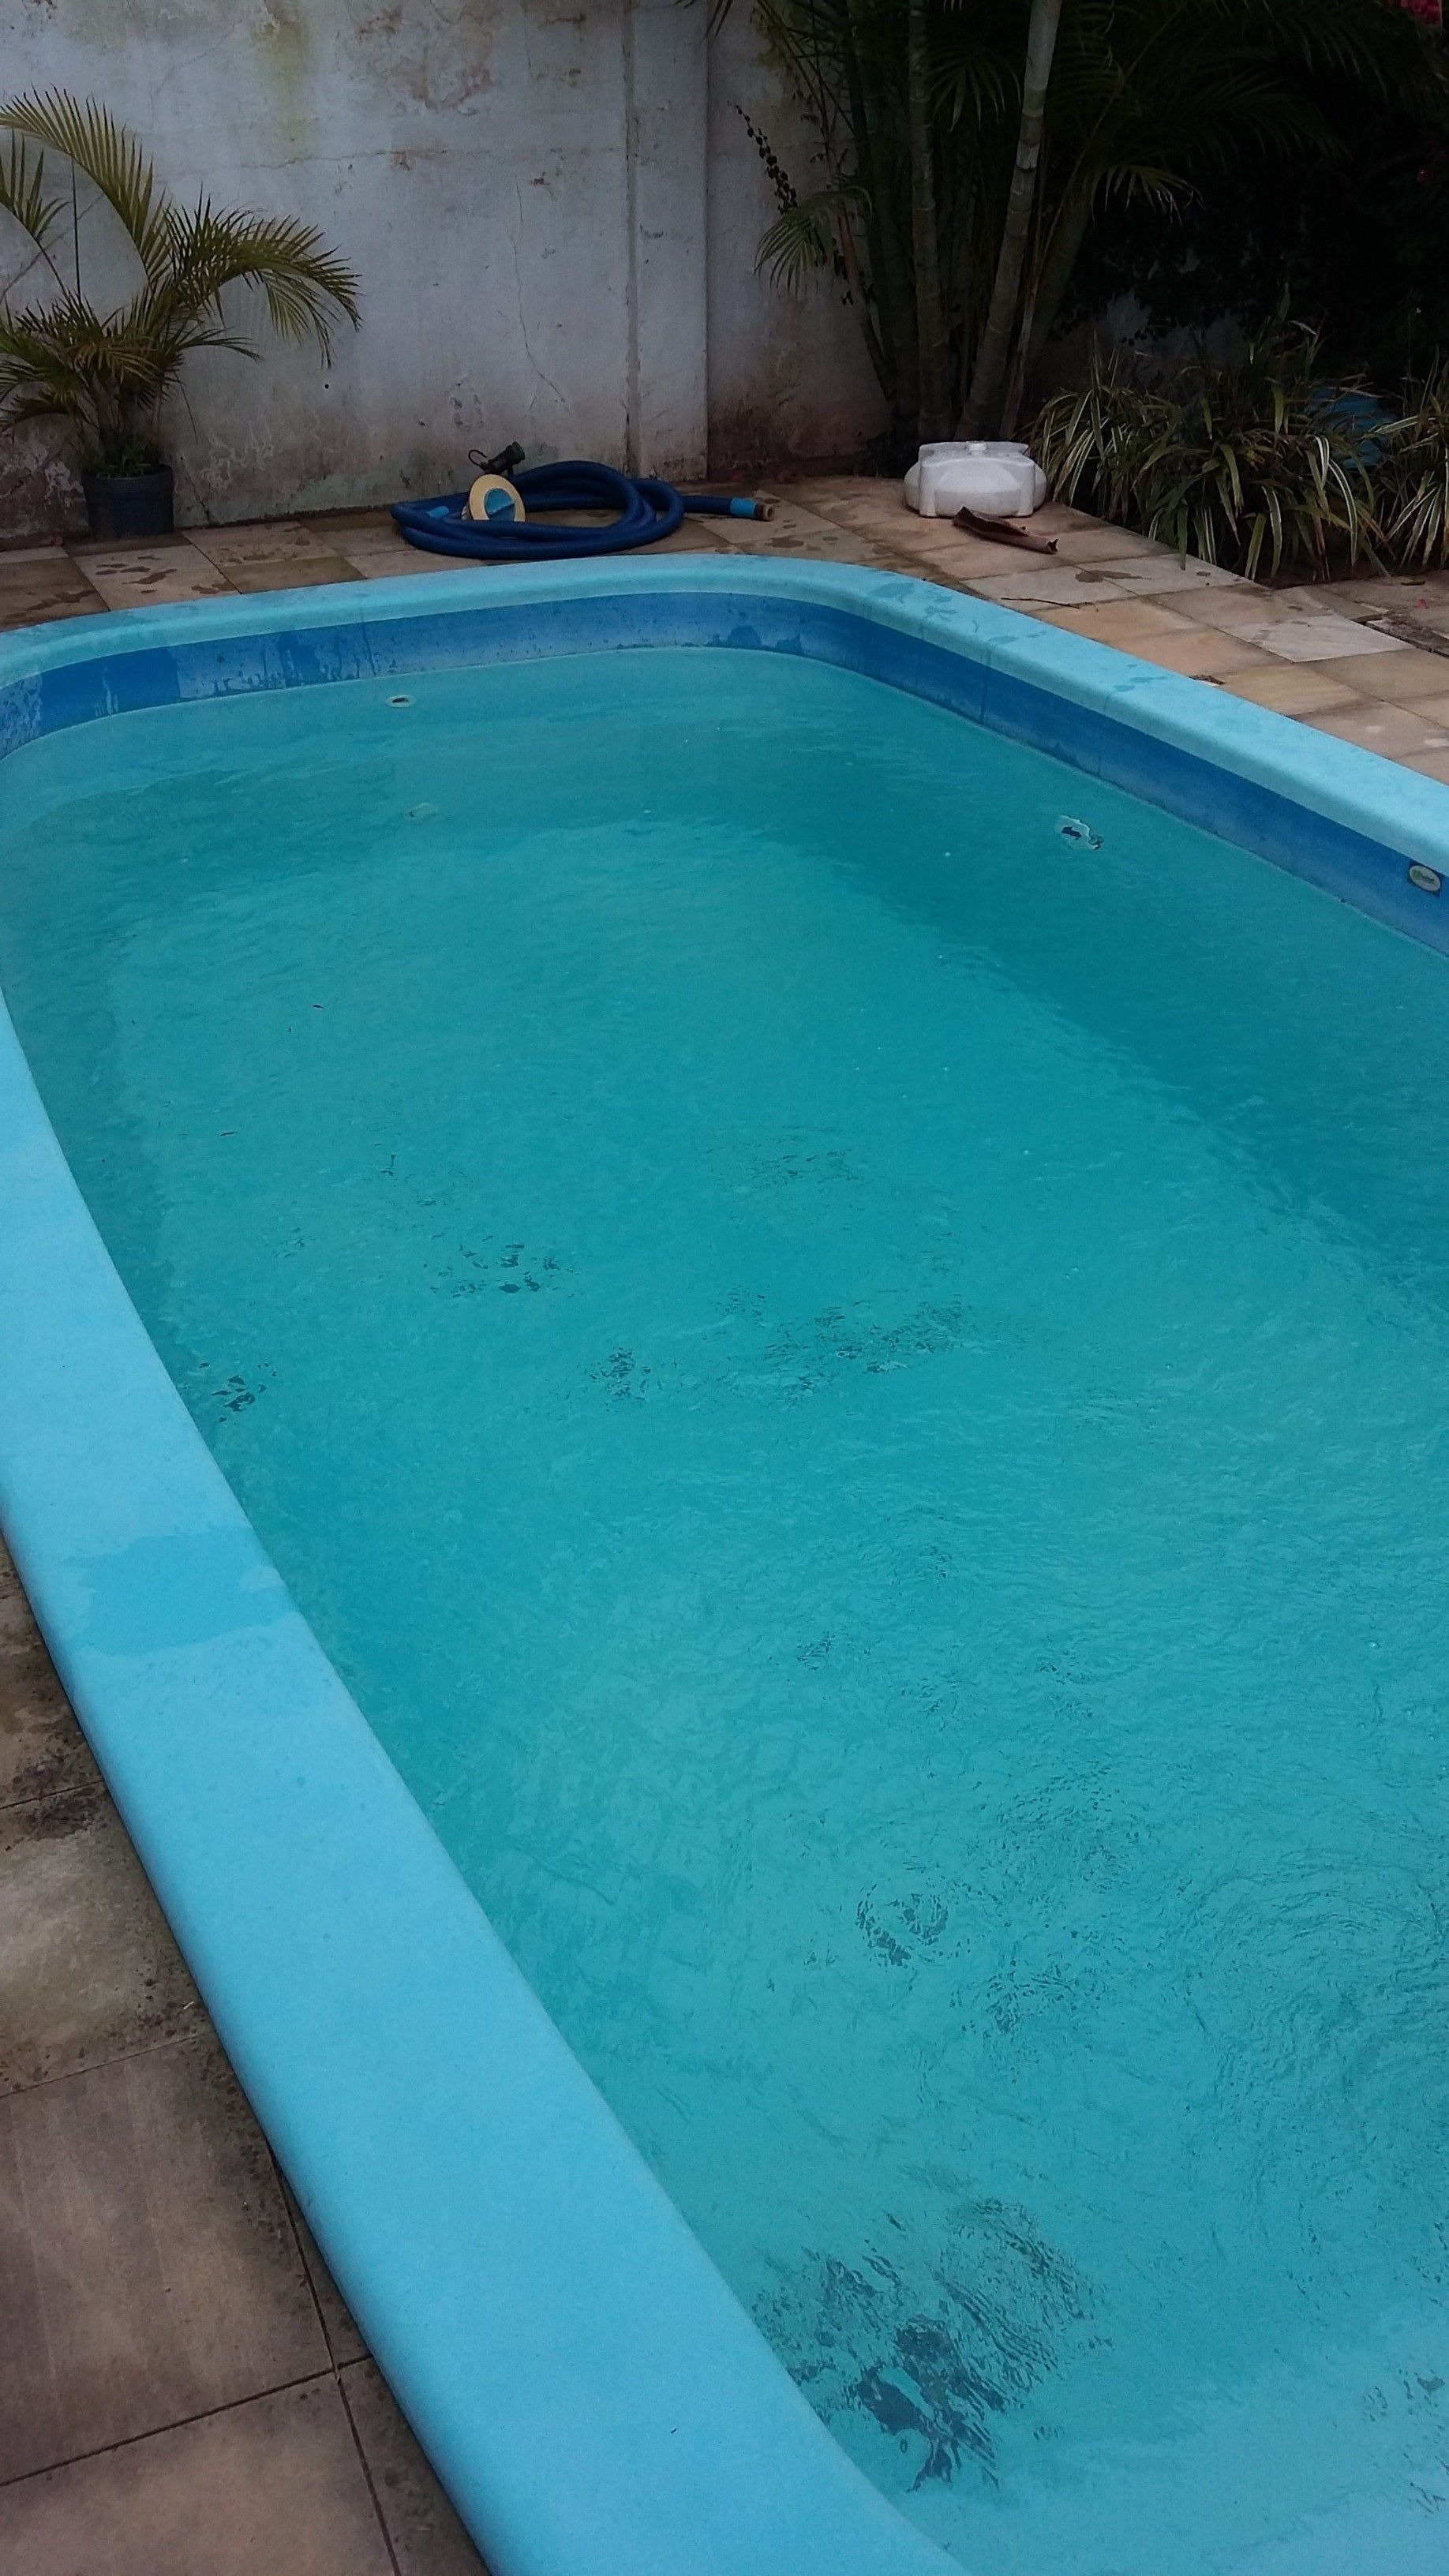
\includegraphics[width=\textwidth]{dados/figuras/piscina_1.jpg}
    \end{subfigure}
    \hspace{1em}
    \begin{subfigure}[t]{0.25\textwidth}
        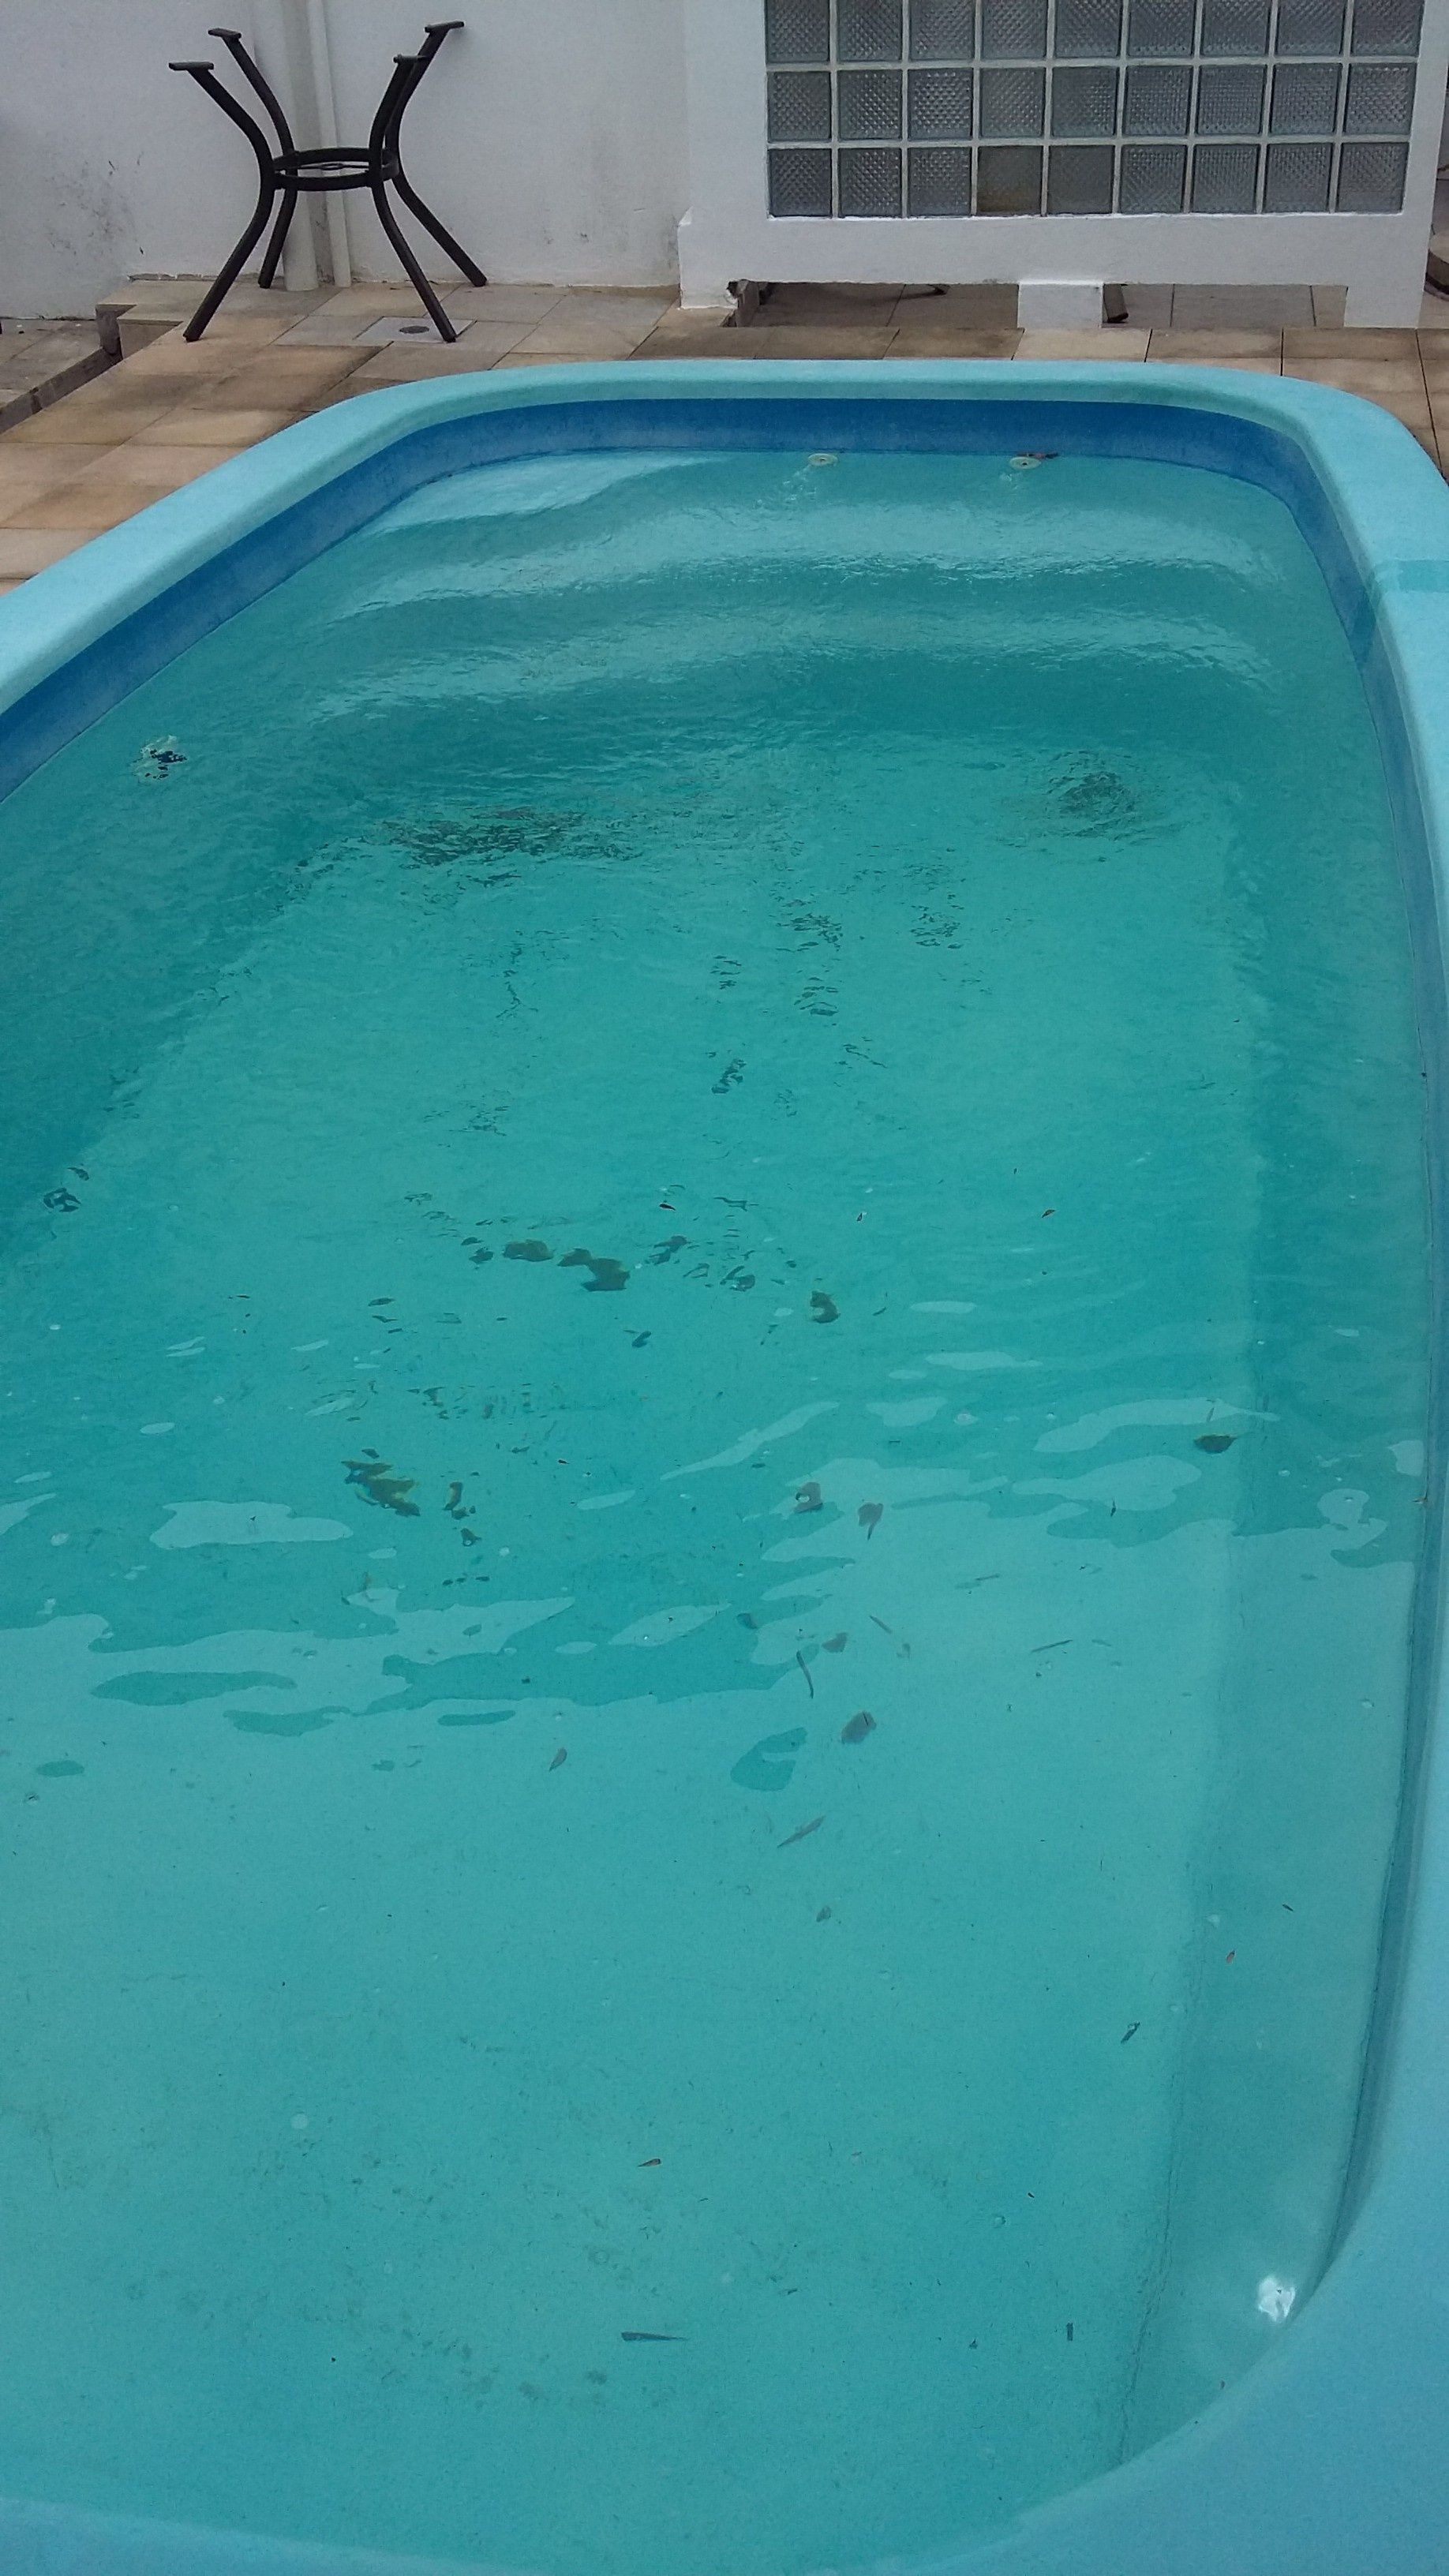
\includegraphics[width=\textwidth]{dados/figuras/piscina_2.jpg}
    \end{subfigure}
\end{figure}

Para fazer a coleta, foi utlizado o ROV, modelo LBV300-5\footnote{Informações completas do modelo do ROV no Anexo \ref{chap:especificacao_rov}.} (Figura \ref{fig:rov_nautec}), do grupo do NAUTEC do C3. 
Acoplado ao robô, será utilizado o sensor MSIS modelo Tritech Micron Sonar\footnote{Informações completas do modelo do sensor no Anexo \ref{chap:especificacao_sonar}.} que é responsável pela captura dos dados.

\begin{figure}[H]
    \centering
    \caption{ROV utilizado no trabalho.}
    \label{fig:rov_nautec}
    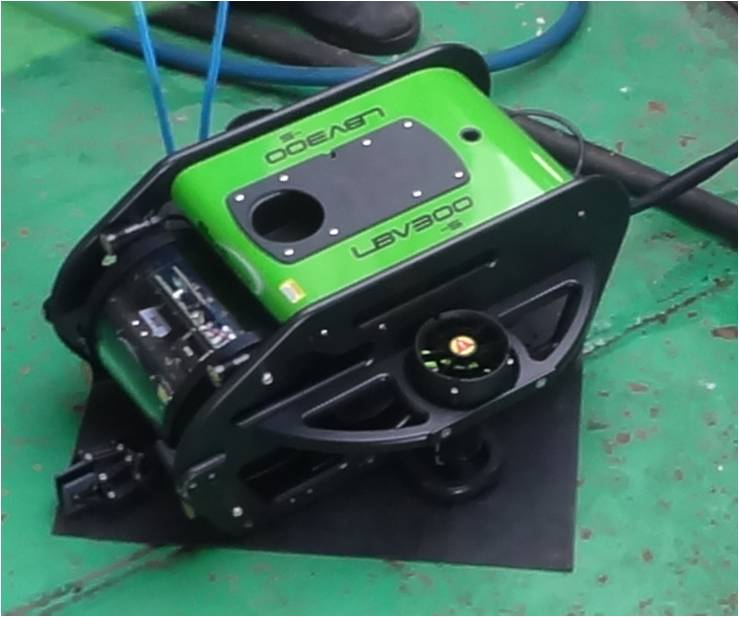
\includegraphics[scale=0.5]{dados/figuras/rov_furg.jpg}
\end{figure}

\section{Pré-processamento}

A etapa de pré-processamento serve para manipular os dados do \textit{dataset} e dispor em uma nuvem de pontos.
No final da fase de pré-processamento, o produto gerado é uma nuvem de pontos da superfície que foi escaneada pelo sonar. Esse resultado servirá como entrada para o próximo processo.

Nessa etapa, ocorre a escolha dos \textit{bins} que vão compor cada imagem.
Deve ser selecionado um \textit{bin} por cada \textit{beam} da imagem acústica.
O critério utilizado será o critério que escolhe o \textit{bin} com o maior sinal de intensidade do \textit{beam}.

\begin{figure}[H]
    \centering
    \caption{Nuvem de pontos gerada a partir de dados coletados em simulação virtual por um sonar MSIS.}
    \label{fig:point_cloud_example}
    \begin{subfigure}[t]{0.45\textwidth}
        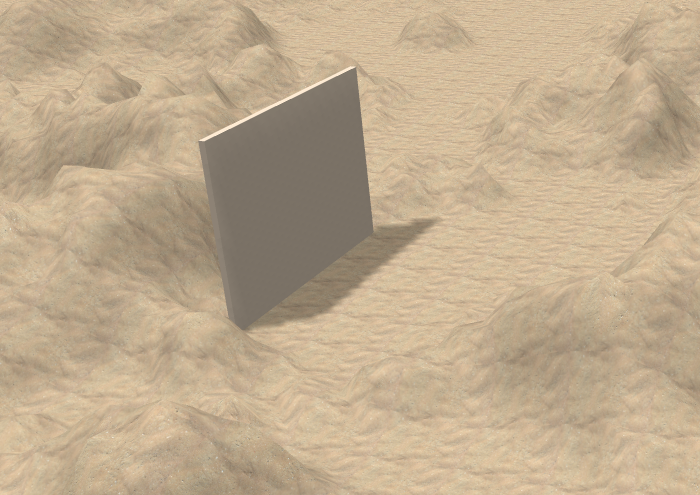
\includegraphics[width=\textwidth]{dados/figuras/scene2.png}
        \caption{Ambiente em simulação virtual.}
        \label{fig:point_cloud_example_a}
    \end{subfigure}
    \begin{subfigure}[t]{0.45\textwidth}
        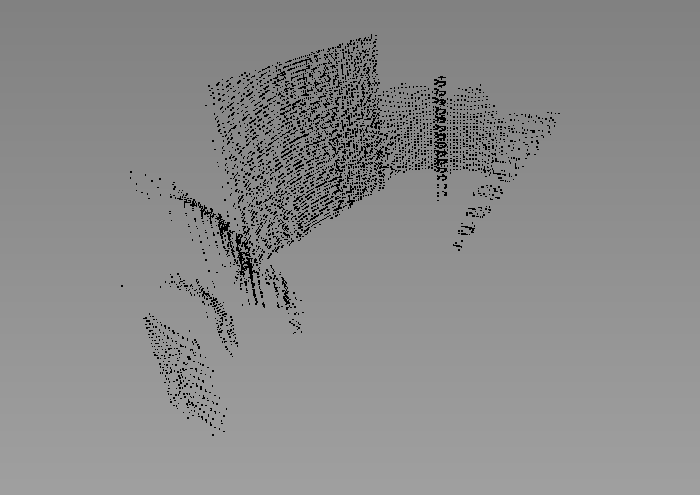
\includegraphics[width=\textwidth]{dados/figuras/point_cloud.png}
        \caption{Nuvem de pontos gerada.}
        \label{fig:point_cloud_example_b}
    \end{subfigure}
\end{figure}

Na Figura \ref{fig:point_cloud_example} mostra o ambiente em simulação escaneado pelo sonar e a nuvem de pontos gerada.
A etapa de pré-processamento não é responsável por filtrar a nuvem de pontos, por esse motivo que a nuvem gerada na Figura \ref{fig:point_cloud_example_b} possui uma grande quantidade de ruído.


\section{Filtragem}
\label{sec:filtragem}

O processo de filtragem ou \textit{denoising} é composto por um conjunto de filtros em forma de funções que tem como objetivo remover ou atenuar informações desnecessárias da nuvem de pontos, como ruídos e \textit{outliers}\footnote{\textit{Outliers} é um termo da área da estatística utilizado para referênciar elementos atípicos ou observações que estão muito afastadas do restante da série.}.
Além disso, o objetivo é facilitar o processo de reconstrução e de cálculo de volume.
O resultado da etapa de filtragem é uma nuvem de pontos mais limpa e legível, porém o processo de filtragem não é capaz de remover todas as informações desnecessárias, como ilustrado na Figura \ref{fig:point_cloud_denoise}.

\begin{figure}[H]
    \centering
    \caption{Processo de remoção de ruído em uma nuvem de pontos.}
    \label{fig:point_cloud_denoise}
    \begin{subfigure}[t]{0.49\textwidth}
        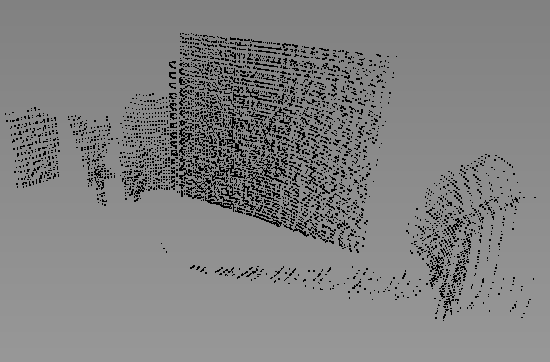
\includegraphics[width=\textwidth]{dados/figuras/pc_noise.png}
        \caption{Nuvem de pontos com ruído.}
    \end{subfigure}
    \begin{subfigure}[t]{0.49\textwidth}
        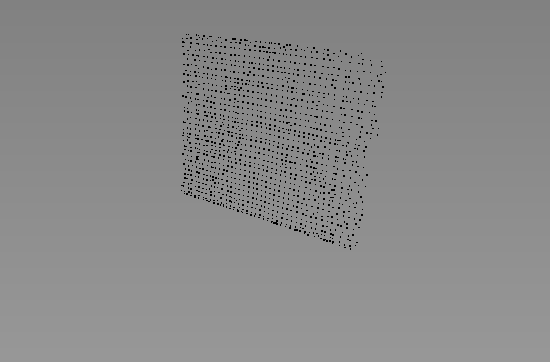
\includegraphics[width=\textwidth]{dados/figuras/pc_denoise.png}
        \caption{Nuvem de pontos após a remoção de ruído.}
    \end{subfigure}
\end{figure}

Para realizar essa etapa, os filtros foram separados em dois grupos.
O primeiro grupo é composto por filtros simples, porém removem maior parte dos pontos desnecessários. 
O segundo conjunto é formado por filtros mais complexos onde muitos já estão implementados na PCL (Seção \ref{sec:pcl}).
Os filtros simples são representados pelo filtro por ângulo, filtro por intensidade e filtro por distância mínima, enquanto que os filtros complexos, são retratados pelo Filtro de Grade de \textit{Voxels}\footnote{Um \textit{voxel} é um \textit{pixel} que contém volume em um espaço tridimensional. Fazendo uma analogia, o \textit{voxel} seria um \textit{pixel} em 3D.}, Filtro de Suavização e o Filtro Estatístico de Remoção de \textit{Outliers}.


\subsection{Filtro por ângulo}
\label{sec:angle_filter}

O filtro por ângulo, remove qualquer ponto que está fora da área cônica definida pelo ângulo horizontal $\theta$. Para esclarecer, na nuvem de pontos da Figura \ref{fig:angle_filter} são mostrados em cinza e em preto, os pontos descartados e mantidos pelo filtro, respectivamente.
O ângulo de abertura no sensor geralmente é configurável no próprio hardware, porém o critério do descarte fica por conta da aplicação, pois em um \textit{dataset}, os mesmos pontos que são inúteis em um trabalho podem ser úteis em outro. 
Por padrão, foi utilizado 120 graus para o ângulo $\theta$.

\subsection{Filtro por distância mínima}
\label{sec:distance_filter}

O filtro por distância mínima faz a remoção de pontos que estão próximos ao sensor, onde a presença de ruído costuma ser elevada. 
Da mesma forma como abordado no filtro anterior, os pontos em cinzas são descartados enquanto que os pretos são mantidos, como mostra a Figura \ref{fig:distance_filter}. 
Por padrão, o valor adotado para o raio de exclusão é de 5\textit{uc}, ou seja, serão descartados todos os pontos que estiverem até 5\textit{uc} de distância do sensor.

\subsection{Filtro por distância máxima}
\label{sec:distance_filter2}

O filtro por distância máxima funciona da mesma forma que o filtro por distância mínima, porém se faz a remoção de pontos que estão distantes do sensor (Figura \ref{fig:distance_filter2}).
Ele é utilizado apenas nos dados coletados no experimento \textit{in loco}, onde a presença de ruído é alta em pontos distantes.

\subsection{Filtro por intensidade}
\label{sec:intensity_filter}

Este processo remove os pontos que possuem baixo valor de intensidade. Os motivos para o sinal de intensidade ser baixo em um determinado ponto, pode ser:
    \begin{itemize}
        \item O ponto estar distante do sensor. Nesse caso, o sinal da onda estará fraco ao entrar em contato com o ponto, por conta da perda de energia para o meio ao longo da distância percorrida;
        \item O ângulo de incidência da onda com o ponto ser obtuso. Quando maior o ângulo de incidência entre a onda e o ponto, mais fraco será o sinal de retorno;
        \item A composição do objeto detectado pela onda. Quanto mais denso for o objeto, maior será o sinal de retorno.
    \end{itemize}

\begin{figure}[H]
    \centering
    \caption{Filtros simples de remoção de \textit{outliers}.}
    \begin{subfigure}[t]{0.4\textwidth}
        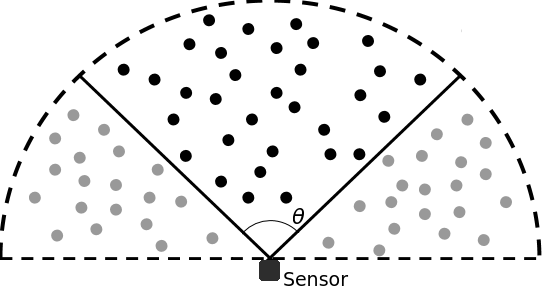
\includegraphics[width=\textwidth]{dados/figuras/angle_filter.png}
        \caption{Filtro por ângulo horizontal.}
        \label{fig:angle_filter}
    \end{subfigure}
    \hspace{3em}
    \begin{subfigure}[t]{0.4\textwidth}
        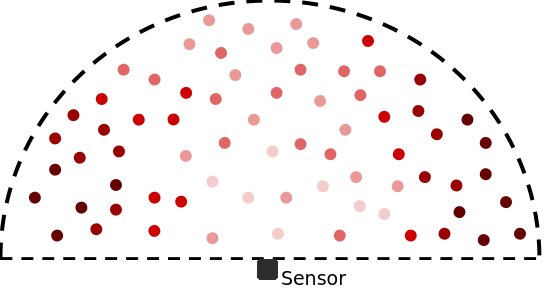
\includegraphics[width=\textwidth]{dados/figuras/intensity_filter.png}
        \caption{Filtro por intensidade.}
        \label{fig:intensity_filter}
    \end{subfigure}
    \begin{subfigure}[t]{0.4\textwidth}
        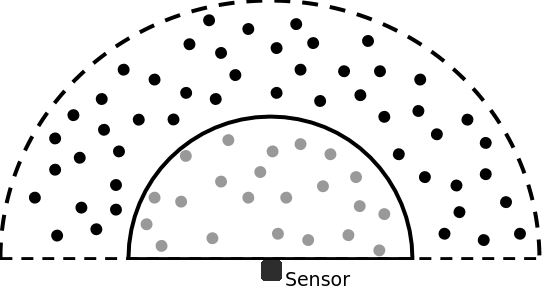
\includegraphics[width=\textwidth]{dados/figuras/distance_filter.png}
        \caption{Filtro por distância mínima.}
        \label{fig:distance_filter}
    \end{subfigure}
    \hspace{3em}
    \begin{subfigure}[t]{0.4\textwidth}
        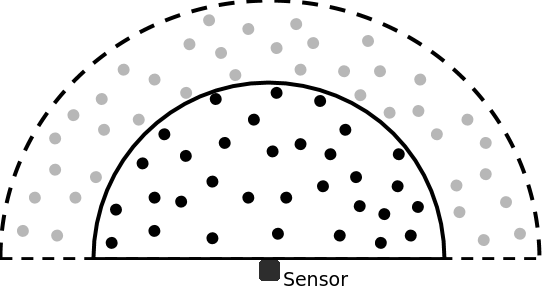
\includegraphics[width=\textwidth]{dados/figuras/distance_filter2.png}
        \caption{Filtro por distância máxima.}
        \label{fig:distance_filter2}
    \end{subfigure}
\end{figure}

O exemplo ilustrado na Figura \ref{fig:intensity_filter}, mostra uma nuvem onde os pontos possuem diversos valores de intensidade. 
Quanto mais claro for o ponto, maior será o seu valor de intensidade do sinal de retorno. 
Portanto, o filtro descarta os pontos mais escuros na imagem.
Por padrão, é descartado todos os pontos que possuírem o valor de intensidade igual ou menor que 5\% da diferença entre o valor máximo e o valor mínimo de intensidade da nuvem de pontos.

\subsection{Filtro de grade de \textit{voxels}}
\label{sec:voxelgrid_filter}

O Filtro de Grade de \textit{Voxels} (do inglês \textit{Voxel Grid Filter}) tem a finalidade de diminuir a resolução/densidade e ordenar os pontos em uma nuvem. 
A Figura \ref{fig:voxelgrid_filter} exibe uma nuvem de pontos de entrada (esquerda) e o resultado gerado após aplicar o filtro (direita).

\begin{figure}[H]
    \centering
    \caption{Exemplo da aplicação do Filtro de Grade de \textit{Voxels}.}
    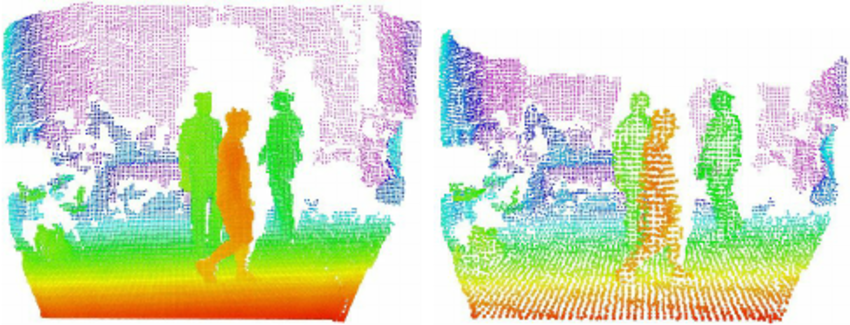
\includegraphics[scale=0.4]{dados/figuras/voxelgrid_filter.png}
    \label{fig:voxelgrid_filter}
    \fonte{\cite{munaro2012tracking}.}
\end{figure}

Para diminuir a quantidade de pontos e ordená-los, o algoritmo cria uma grade no conjunto de dados, onde os pontos são deslocados para o centroide da célula (\textit{voxel}) da grade em que estão contidos (o tamanho do \textit{voxel} é definido pelo usuário). A diminuição da quantidade e ordenação dos pontos facilita o processo de triangularização (etapa posterior responsável por transformar a nuvem de pontos em uma superfície).

\subsection{Filtro estatístico de remoção de \textit{outliers}}
\label{sec:statistical_outlier_removal}

O SORF (Filtro Estatístico de Remoção de \textit{Outliers}, do inglês \textit{Statistical Outlier Removal Filter}) é um filtro da biblioteca PCL que é responsável por remover conjuntos de pontos que possuem uma densidade menor do que o restante dos conjuntos de pontos dentro da nuvem. 
A Figura \ref{fig:outlier_filter} exemplifica a aplicação do filtro. Na imagem à esquerda mostra a nuvem original que contém regiões em destaque, onde a densidade de pontos é menor que no restante da nuvem, enquanto que na imagem à direita mostra a remoção desses conjuntos de pontos.

\begin{figure}[H]
    \centering
    \caption{Exemplo de uso do SORF.}
    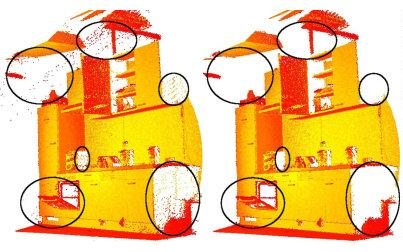
\includegraphics[scale=0.6]{dados/figuras/outlier_filter.jpg}
    \fonte{Adaptado de \cite{rusu2011pcl}.}
    \label{fig:outlier_filter}
\end{figure}

O filtro percorre a nuvem calculando, para cada ponto, a distância média entre seus pontos vizinhos (o número de vizinhos é definido pelo usuário). Assumindo o resultado como uma distribuição Gaussiana com uma média e um desvio padrão, todos os pontos cuja distância média estão fora de um intervalo definido pela média das distâncias globais e desvio padrão podem ser considerados \textit{outliers} e, portanto, removidos do conjunto de dados.

\subsection{Filtro de suavização}
\label{sec:smoothing_filter}

O Filtro de Suavização é um filtro que está presenta na biblioteca PCL e é responsável por suavizar e reconstruir a superfície de pontos na nuvem. 
Para realizar o procedimento, o filtro utiliza o MLS (do inglês \textit{Moving Least Squares}), um método de reamostragem, desenvolvido por \cite{levin1998mls}, capaz de recriar partes ausentes ou suavizar superfícies por meio da interpolação polinomial entre pontos. 
Para exemplificar, a Figura \ref{fig:smoothing_filter} exibe uma superfície sem tratamento (imagem à esquerda) e a mesma superfície após a aplicação do filtro (imagem à direita).

\begin{figure}[H]
    \centering
    \caption{Exemplo do uso do Filtro de Suavização.}
    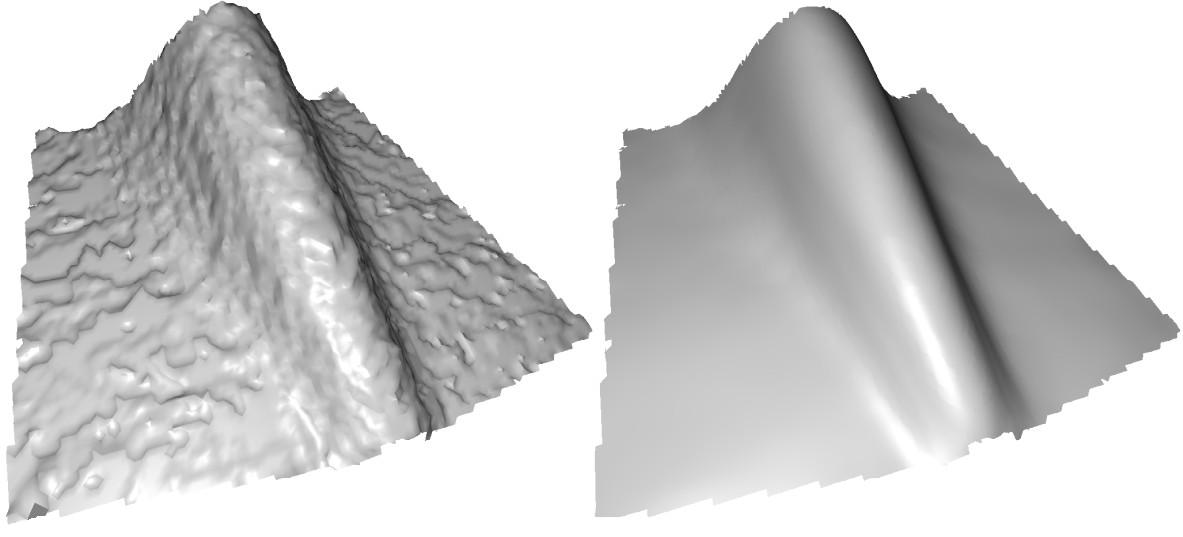
\includegraphics[scale=0.3]{dados/figuras/mls_filter.jpg}
    \fonte{Adaptado de \cite{ridel2015mls}.}
    \label{fig:smoothing_filter}
\end{figure}

No trabalho, o filtro é utilizado com o intuito de suavizar e corrigir boa parte do ruído e pequenos erros de medição de distância gerado nos dados, provenientes da movimentação do robô enquanto realiza a coleta.

\section{Reconstrução}
\label{sec:reconstrucao}

A reconstrução do modelo tridimensional é gerada a partir da nuvem de pontos, onde é obtido a forma final da superfície. 
Como exemplo, a Figura \ref{fig:reconstruction} mostra a reconstrução de um objeto passo a passo.

\begin{figure}[H]
    \centering
    \caption{Reconstrução de um objeto em 3D a partir de uma nuvem de pontos.}
    \label{fig:reconstruction}
    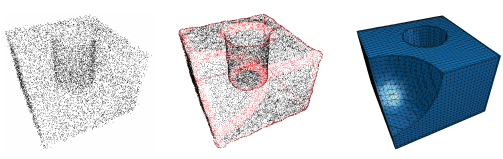
\includegraphics[scale=0.8]{dados/figuras/reconstruction.png}
    \fonte{Adaptado de \cite{jenke2006bayesian}.}
\end{figure}

Para dar forma à superfície é necessário uma lógica para ligar os pontos, para tal lógica chamamos de triangulação.
No trabalho, a triangulação é feita através da construção de triângulos sem fazer sobreposições. 
Apesar do nome triangulação remeter à triângulos, ela pode ser constituída por qualquer espaço em simplexos ou em polígonos. 
Os simplexos são extensões de triângulos em outras dimensões, tais como segmentos de reta, tetraedros, triângulos e etc. 
Os elementos que constituem uma triangulação, são denominados de face.
A Figura \ref{fig:triangulation} mostra algumas formas para fazer a triangulação em um conjunto de pontos, como a triangulação incremental e a triangulação do fecho convexo.

\begin{figure}[H]
    \centering
    \caption{Exemplos de modelos de triangulação.}
    \begin{subfigure}[t]{0.6\textwidth}
        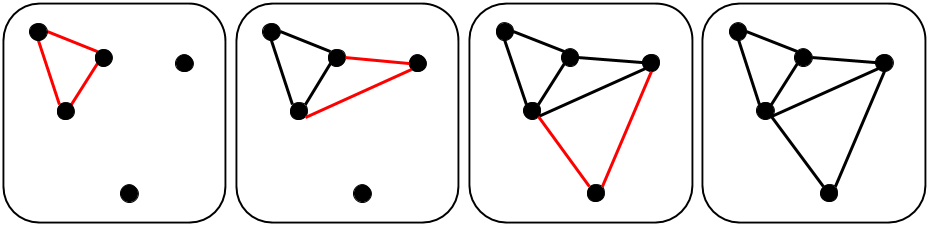
\includegraphics[width=\textwidth]{dados/figuras/triangulation_incremental.png}
        \caption{Triangulação Incremental}
        \label{fig:incremental_triangulation}
    \end{subfigure}
    \hspace{5em}
    \begin{subfigure}[t]{0.6\textwidth}
        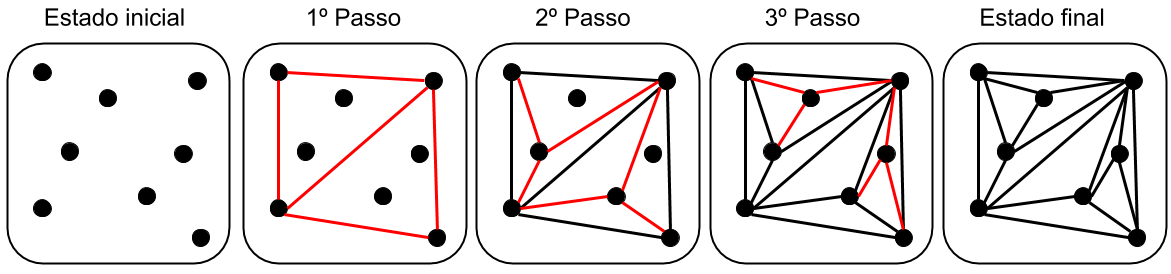
\includegraphics[width=\textwidth]{dados/figuras/triangulation_convex.png}
        \caption{Triangulação do Fecho Convexo}
        \label{fig:convex_triangulation}
    \end{subfigure}
    \label{fig:triangulation}
\end{figure}

Na Figura \ref{fig:incremental_triangulation} mostra a triangulação incremental, onde é realizada a construção de triângulos a partir da seleção aleatória do ponto inicial, seguindo a ligação pelo ponto mais próximo. 
Na Figura \ref{fig:convex_triangulation} mostra a triangulação do fecho convexo, na qual se realiza o fecho convexo do conjunto de pontos seguindo pela triangulação.
Após esse primeiro passo, para cada ponto no interior dos triângulos formados, se divide em mais três triângulos.

Fecho convexo (também conhecido como invólucro convexo ou envoltório convexo) são estruturas que englobam o conjunto de pontos, através da intersecção com seus pontos marginais. No plano, o fecho convexo é um polígono, enquanto que no espaço é representado por uma superfície (Figura \ref{fig:convex_hull}).

\begin{figure}[H]
    \centering
    \caption{Fecho convexo representado no plano (esquerda) e no espaço (direita).}
    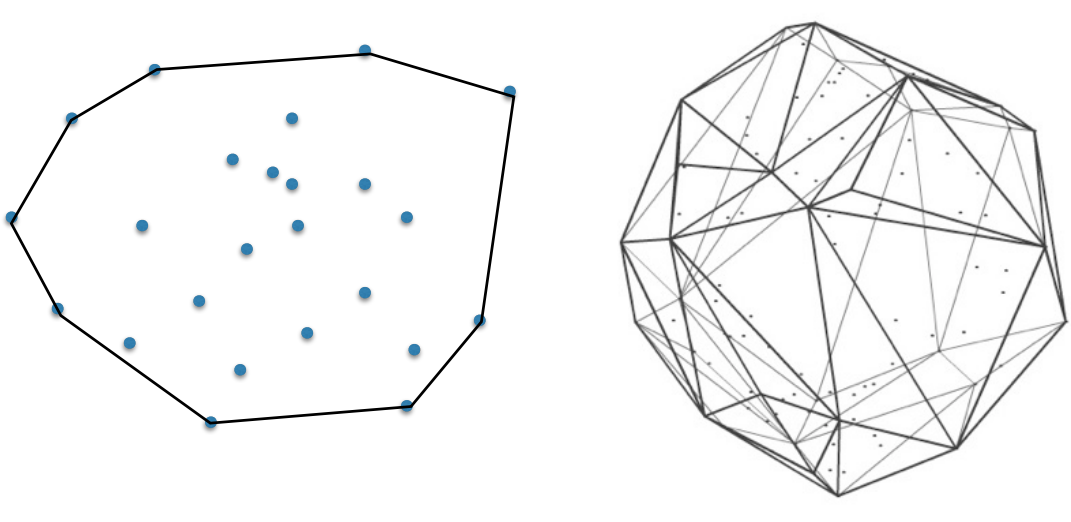
\includegraphics[scale=0.4]{dados/figuras/convex_hull.png}
    \label{fig:convex_hull}
\end{figure}

Uma triangulação nem sempre é adequada para um certo problema, pois os triângulos precisam ser semelhantes com o triângulo equilátero (triângulos que não possuem ângulos internos agudos). Essas triangulações especiais usam critérios para definir triângulos, entre os modelos conhecidos existe a Triangulação de Delaunay.


\subsection{Triangulação de Delaunay}
\label{sec:delaunay}
A triangulação de Delaunay, proposto por \cite{delaunay1934sphere}, é o método responsável por fornecer uma triangulação com o maior ângulo mínimo, ou seja, os melhores triângulos de forma única, em um determinado conjunto de pontos. O método pode ser formulado e estudado no espaço euclidiano de dimensão $n$, mas para fins didáticos será definida e exemplificada apenas no plano.

\begin{figure}[H]
    \centering
    \caption{(a) Triangulação que não satisfaz o critério de Delaunay; (b) Triangulação de Delaunay.}
    \begin{subfigure}[t]{0.2\textwidth}
        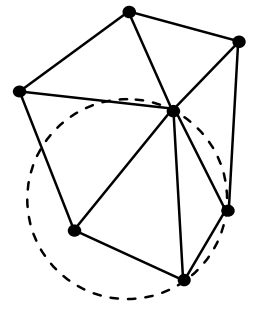
\includegraphics[width=\textwidth]{dados/figuras/delaunay1.png}
        \caption{}
        \label{fig:delaunay1}
    \end{subfigure}
    \hspace{3em}
    \begin{subfigure}[t]{0.3\textwidth}
        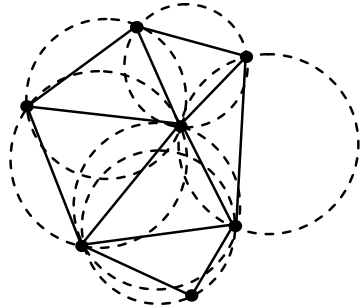
\includegraphics[width=\textwidth]{dados/figuras/delaunay2.png}
        \caption{}
        \label{fig:delaunay2}
    \end{subfigure}
    \fonte{Adaptado de \cite{piteri2007triangulacao}.}
    \label{fig:delaunay}
\end{figure}

Para a criação dos triângulos, se pode utilizar qualquer metodologia de triangulação (inclusive as que foram apresentadas na Figura \ref{fig:triangulation}). Após a criação, há uma verificação, que deve ser realizada em cada triângulo da malha, definida pela regra do circuncirculo, que determina se o triângulo é ou não de Delaunay. 
A regra descreve que para cada triângulo da malha, é traçado um círculo que passa pelos três vértices do triângulo, se esse círculo conter apenas os 3 pontos do triângulo, então ele satisfaz a regra. 
Se haver mais de 3 pontos dentro, então é aplicada a troca (\textit{flip}) entre arestas contidas no círculo.

Para explicar o termo \textit{flip}, observe a Figura \ref{fig:delaunay1}, onde o triângulo ABC não satisfaz a regra do circuncirculo, pois há outro vértice contido (D).
Para resolver esse problema se utiliza o \textit{flip} entre os triângulos ABC e ACD, que faz a troca da aresta AC pela aresta DB. 
Refazendo a regra do circuncirculo nos triângulos, é possível observar (Figura \ref{fig:delaunay2}) que ambos agora são triângulos de Delaunay.

Na Figura \ref{fig:delaunay_theorem} há outro exemplo de \textit{flip}. A Figura \ref{fig:delaunay_theorem2} mostra ambos triângulos que não obedecem a regra do circuncírculo. Realizando o \textit{flip} entre as arestas BD e AC, a regra se torna válida (Figura \ref{fig:delaunay_theorem3}). 

\begin{figure}[H]
    \centering
    \caption{Regra do circuncírculo que define se um triângulo é ou não de Delaynay.}
    \begin{subfigure}[t]{0.2\textwidth}
        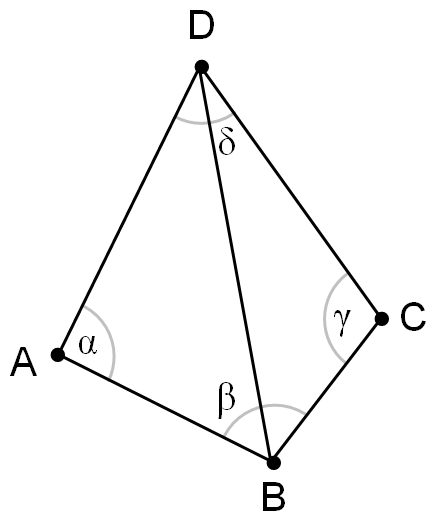
\includegraphics[width=\textwidth]{dados/figuras/delaunay_theorem1.png}
        \caption{}
        \label{fig:delaunay_theorem1}
    \end{subfigure}
    \hspace{2em}
    \begin{subfigure}[t]{0.27\textwidth}
        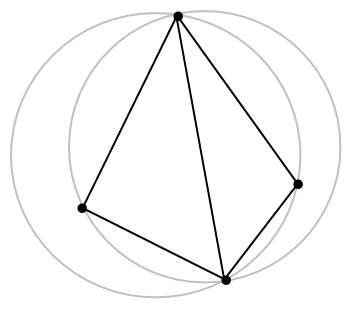
\includegraphics[width=\textwidth]{dados/figuras/delaunay_theorem2.png}
        \caption{}
        \label{fig:delaunay_theorem2}
    \end{subfigure}
    \hspace{2em}
    \begin{subfigure}[t]{0.2\textwidth}
        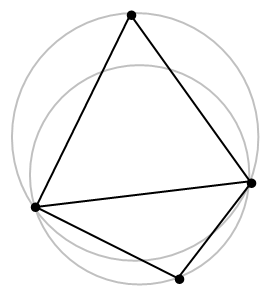
\includegraphics[width=\textwidth]{dados/figuras/delaunay_theorem3.png}
        \caption{}
        \label{fig:delaunay_theorem3}
    \end{subfigure}
    \label{fig:delaunay_theorem}
\end{figure}

Para realizar uma triangulação de um conjunto de pontos que estão dispersos pelo espaço é necessário projetá-los em um mesmo plano, pois só assim é possível reconstruir uma superfície aberta\footnote{Entende-se como superfície aberta qualquer forma ou geometria no espaço, no qual não possui volume, possui um ponto inicial e final e ambos pontos não se conectam. Uma superfície fechada possui um volume, que é o caso da esfera, do cubo, do torom etc.}.
Após a criação das faces, os pontos retornam para o espaço 3D.
Contudo, algumas faces podem conter pontos que estejam próximos no momento da triangulação no plano, mas distantes no espaço 3D, ocasionando em triângulos com uma grande área e que podem estar sobrepondo outros triângulos. 
Esse problema será tratado na próxima seção (Seção \ref{sec:split_mesh}).
Na Figura \ref{fig:prism} é possível observar uma projeção de pontos e faces em um plano.


\subsection{Separação da superfície}
\label{sec:split_mesh}

A separação da superfície é um processo que faz a divisão da malha e remove as sub-malhas desnecessárias, além de corrigir erros de reconstrução.
Essa etapa ocorre dentro da etapa de reconstrução e faz a utilização da biblioteca Pymesh (descrita na Seção \ref{sec:pymesh}).

Como visto na seção anterior, a etapa de triangulação de uma nuvem de pontos no plano pode criar triângulos sobrepostos e com uma grande área (Figura \ref{fig:split_mesh2}).
Para resolver esse problema, é necessário definir um valor para a  área máxima do triângulo, ou seja, se a área do triângulo criado for maior que o valor definido de área máxima, então essa face é descartada da malha.
O valor definido para a área máxima pode depender do tamanho e da densidade da nuvem de pontos.
Essa abordagem resolve o problema, porém com o descarte de faces, acaba surgindo lacunas e descontinuidades na malha, gerando sub-malhas (Figura \ref{fig:split_mesh3}).

\begin{figure}[H]
    \centering
    \caption{Processo de remoção das sub-malhas.}
    \begin{subfigure}[t]{0.4\textwidth}
        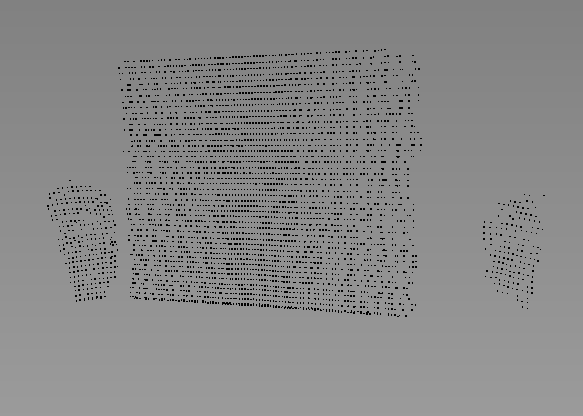
\includegraphics[width=\textwidth]{dados/figuras/split_mesh1.png}
        \caption{Nuvem de pontos antes da reconstrução.}
        \label{fig:split_mesh1}
    \end{subfigure}
    \begin{subfigure}[t]{0.4\textwidth}
        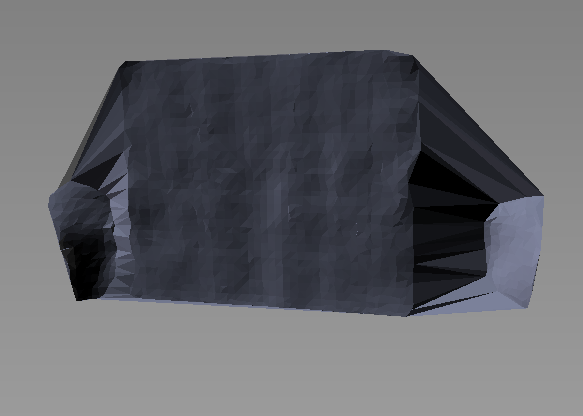
\includegraphics[width=\textwidth]{dados/figuras/split_mesh2.png}
        \caption{Superfície sem aplicar a separação.}
        \label{fig:split_mesh2}
    \end{subfigure}
    \begin{subfigure}[t]{0.4\textwidth}
        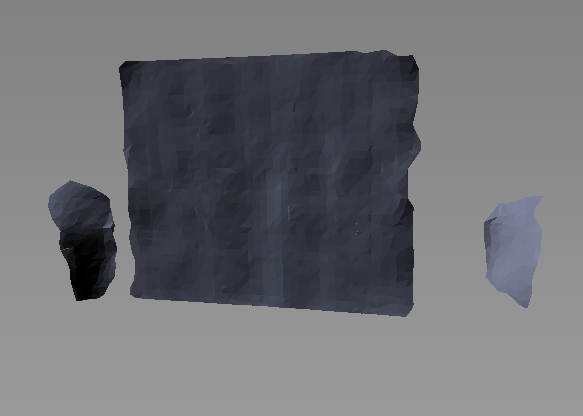
\includegraphics[width=\textwidth]{dados/figuras/split_mesh3.png}
        \caption{Superfície após a remoção dos grandes triângulos.}
        \label{fig:split_mesh3}
    \end{subfigure}
    \begin{subfigure}[t]{0.4\textwidth}
        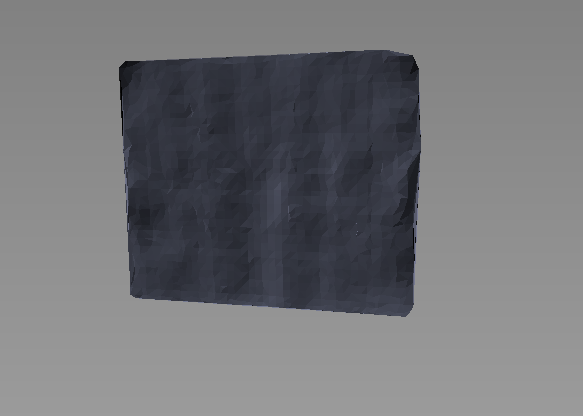
\includegraphics[width=\textwidth]{dados/figuras/split_mesh4.png}
        \caption{Superfície após a remoção das sub-malhas.}
        \label{fig:split_mesh4}
    \end{subfigure}
    \label{fig:split_mesh}
\end{figure}

Para escolher a sub-malha que represente melhor a superfície escaneada pelo sensor, se faz o cálculo de área de cada sub-malha.
Aquela que apresentar maior área será escolhida e o restante será descartado (Figura \ref{fig:split_mesh4}).


\section{Comparação}
\label{sec:comparacao}

A comparação é a última etapa do processo de desenvolvimento. 
Essa parte é possível fazer a comparação entre dois modelos e determinar o quanto se perdeu ou ganhou em relação ao volume e superfície. 
A principal aplicação é modelar coletas do mesmo local em diferentes períodos e fazer a comparação entre os resultados alcançados.

Os resultados são obtidos a partir da diferença entre dois modelos reconstruídos, por esse motivo a etapa de comparação é um processo separado do restante. 
O cálculo de superfície ocorre nas etapas de reconstrução e comparação, enquanto que o cálculo de volume só ocorre na etapa de comparação, por esse motivo ambos serão descritos nessa seção.

\subsection{Cálculo de superfície}
\label{sec:surface_calc}

O cálculo da área de superfície é importante para estimar a qualidade da reconstrução.
A superfície é uma malha de triângulos, portanto para calcular a área total, basta somar a área de cada triângulo contido nela. 
Para esse tipo de cálculo foi utilizada a fórmula de Heron (ou de Herão), que é capaz de calcular a área de qualquer tipo de triângulo em função das medidas dos seus três lados.
A fórmula de Heron é mostrada pela Equação \ref{eq:heron}, onde $a$, $b$ e $c$ são os três lados e $p$ representa o semiperímetro do triângulo (Equação \ref{eq:heron_p}).

\begin{equation}
    \label{eq:heron}
    A = \sqrt{p(p-a)(p-b)(p-c)}
\end{equation}

\begin{equation}
    \label{eq:heron_p}
    p = \frac{a+b+c}{2}
\end{equation}


\subsection{Cálculo de volume}
\label{sec:volume_calc}

O processo de cálculo de volume é fundamental para realizar a comparação entre reconstruções.
O volume é formado a partir da projeção da superfície do modelo em um plano base, como mostra na Figura \ref{fig:prism}.
O resultado da projeção é um conjunto de poliedros irregulares, onde cada poliedro possui uma base inferior diferente da base superior.

\begin{figure}[H]
    \centering
    \caption{Formação do volume a partir da superfície.}
    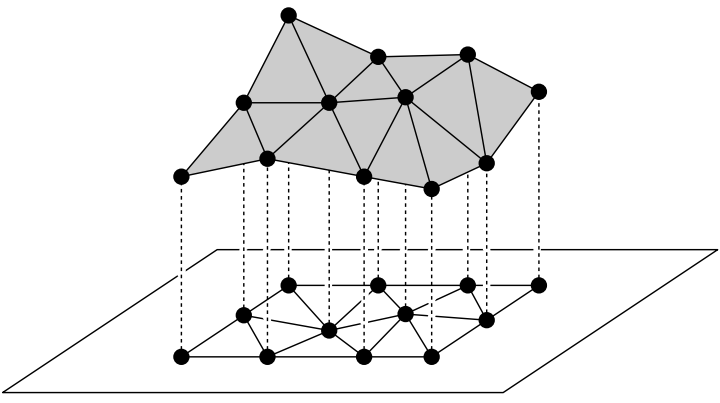
\includegraphics[scale=0.5]{dados/figuras/prisms.png}
    \fonte{\cite{berg2008computational}}
    \label{fig:prism}
\end{figure}

O plano base em uma comparação é definido pelo ponto mais distante do sensor entre os dois modelos.
Com o ponto selecionado, o plano base é traçado e ambos modelos constroem seus volumes com base nesse plano, como mostra a Figura \ref{fig:projection}.

\begin{figure}[H]
    \centering
    \caption{Reconstrução do volume de dois modelos em comparação.}
    \begin{subfigure}[t]{0.325\textwidth}
        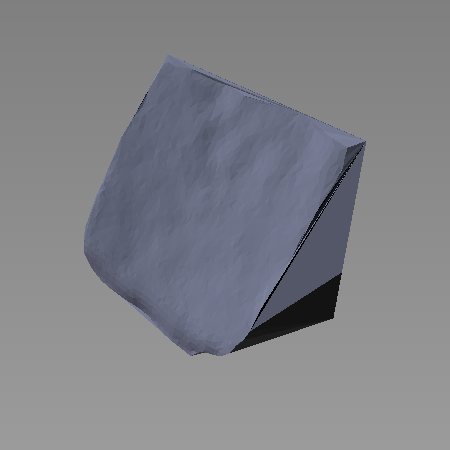
\includegraphics[width=\textwidth]{dados/figuras/projection1.png}
        \caption{Volume que possui o ponto mais distante do sensor.}
        \label{fig:projection1}
    \end{subfigure}
    \begin{subfigure}[t]{0.325\textwidth}
        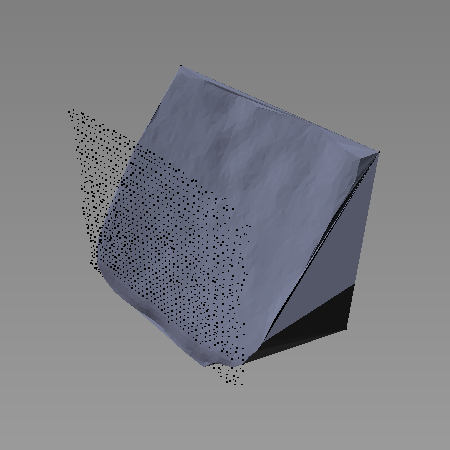
\includegraphics[width=\textwidth]{dados/figuras/projection2.png}
        \caption{Comparação entre modelos.}
        \label{fig:projection2}
    \end{subfigure}
    \begin{subfigure}[t]{0.325\textwidth}
        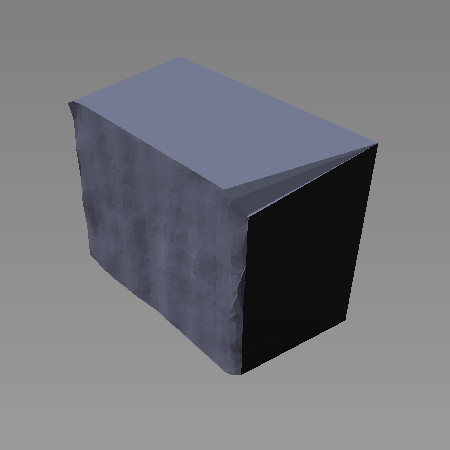
\includegraphics[width=\textwidth]{dados/figuras/projection3.png}
        \caption{Geração do volume do segundo modelo.}
        \label{fig:projection3}
    \end{subfigure}
    \label{fig:projection}
\end{figure}

O poliedro irregular é semelhante ao prisma regular, porém suas bases são diferentes (Figura \ref{fig:polyhedron}). Por esse motivo, não se pode utilizar a fórmula convencional de cálculo de volume de prismas regulares.  
Porém, apesar de ser pouco provável, pode haver poliedros com a forma de um prisma regular (quando os 3 pontos da base superior se encontram na mesma altura). 
O algoritmo é capaz de tratar esse caso específico.

\begin{figure}[H]
    \centering
    \caption{Exemplo de um poliedro irregular.}
    \begin{subfigure}[t]{0.25\textwidth}
        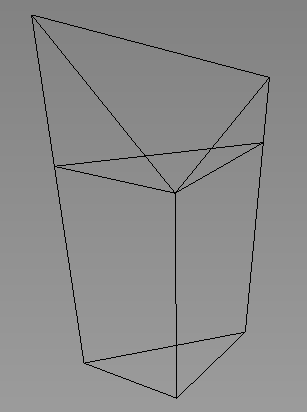
\includegraphics[width=\textwidth]{dados/figuras/pol_line.png}
        \caption{Poliedro em faces.}
        \label{fig:polyhedron1}
    \end{subfigure}
    \hspace{2em}
    \begin{subfigure}[t]{0.25\textwidth}
        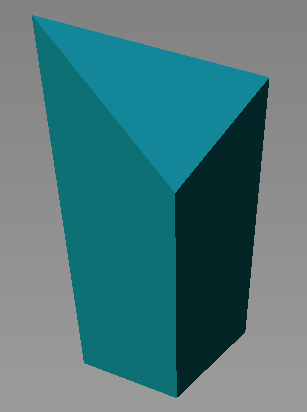
\includegraphics[width=\textwidth]{dados/figuras/pol_solid.png}
        \caption{Poliedro em sólido.}
        \label{fig:polyhedron2}
    \end{subfigure}
    \hspace{2em}
    \begin{subfigure}[t]{0.25\textwidth}
        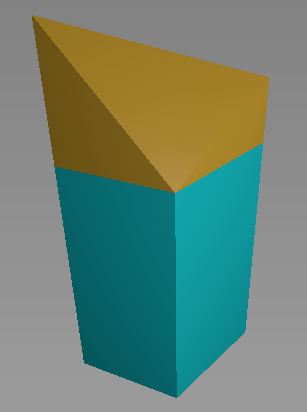
\includegraphics[width=\textwidth]{dados/figuras/pol_sep.png}
        \caption{Prisma e pirâmide destacados.}
        \label{fig:polyhedron3}
    \end{subfigure}
    \label{fig:polyhedron}
\end{figure}

Antes de realizar o procedimento, é importante saber que os dados utilizados como parâmetros são 6 pontos, sendo os 3 pontos da base inferior e os 3 pontos da base superior do poliedro irregular.
Para realizar esse cálculo, é necessário dividir o poliedro irregular na altura do ponto da base superior mais próximo à base inferior.
O resultado da divisão é uma pirâmide irregular na parte superior e um prisma regular na parte inferior, como ilustra a Figura \ref{fig:polyhedron3}.
Os pontos $b$ e $e$ são projeções dos pontos $a$, $c$ e $d$, ilustrado na Figura \ref{fig:pyramid_i}.

\begin{figure}[H]
    \centering
    \caption{Poliedro separado em dois volumes.}
    \begin{subfigure}[t]{0.3\textwidth}
        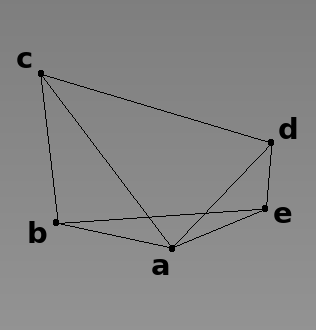
\includegraphics[width=\textwidth]{dados/figuras/pyramid_line3.png}
        \caption{Pirâmide irregular.}
        \label{fig:pyramid_i}
    \end{subfigure}
    \hspace{2em}
    \begin{subfigure}[t]{0.3\textwidth}
        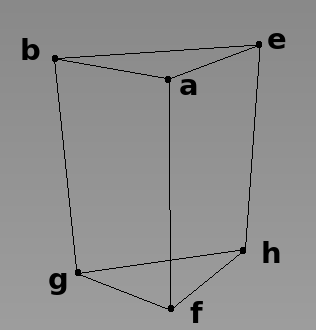
\includegraphics[width=\textwidth]{dados/figuras/prism_line2.png}
        \caption{Prisma regular.}
        \label{fig:prism_i}
    \end{subfigure}
\end{figure}

A separação torna o cálculo do volume mais simples, como mostra a Equação \ref{eq:volume_polyhedron}. 
O volume total ($V_t$) é composto pela soma do volume da pirâmide ($V_{pi}$) com o volume do prisma ($V_{pr}$).
Na Equação \ref{eq:volume_pyramid}, o volume do prisma é $1/3$ do produto da base ($b_{pi}$) pela altura ($h_{pi}$). 
Por fim, o volume da pirâmide é o produto da base ($b_{pr}$) pela altura  ($h_{pr}$), como mostra a Equação \ref{eq:volume_prism}.
A área da base da pirâmide é um trapézio retângulo e é descrita pela Fórmula \ref{eq:trap_rect}, onde $B$ é a base maior ($\left | \overrightarrow{cb} \right |$)), $b$ é a base menor ($\left | \overrightarrow{de} \right |$)) e $h$ é a distância entre as bases ($\left | \overrightarrow{be} \right |$)


\begin{multicols}{3}
    \begin{equation}
        \label{eq:volume_polyhedron}
        V_t = V_{pr} + V_{pi}
    \end{equation}
    \begin{equation}
        \label{eq:volume_pyramid}
        V_{pr} = b_{pr} \cdot h_{pr}
    \end{equation}
    \begin{equation}
        \label{eq:volume_prism}
        V_{pi} = \frac{1}{3} \cdot b_{pi} \cdot h_{pi}
    \end{equation}
\end{multicols}

\begin{equation}
    \label{eq:trap_rect}
    b_{pi} = (B+b) \cdot h \cdot \frac{1}{2}
\end{equation}
\vspace{0.5em}

\iffalse
O Algoritmo \ref{alg:poly_alg} descreve o procedimento para o cálculo de volume de um poliedro irregular. 
O parâmetro de entrada são dois conjuntos de pontos que representam o triângulo da base inferior ($T_{inf}$) e o triângulo da base superior ($T_{sup}$).
Suponto que $p_a$ é o ponto mais próximo ao plano base, $p_b$ e $p_e$ são projeções dos pontos $p_c$, $p_d$ e $p_a$ (como ocorre no exemplo da Figura \ref{fig:pyramid_i}).

\vspace{1em}
\begin{algorithm}[H]
    \caption{Cálculo de Volume de um Poliedro Irregular}
    \hspace{1em}
    \KwIn{$T_{inf}$, $T_{sup}$}
    \KwOut{$V_t$}
    \For {$ponto \in T_{sup}$} {
        \If {$ponto$ for mais próximo ao plane base} {
            $p_a \leftarrow ponto$ \\
        }
    }
    $p_b \leftarrow$ proj($p_a$, $p_c$) \\
    $p_e \leftarrow$ proj($p_a$, $p_d$) \\
    
    $b_{pi} \leftarrow$ AreaBasePiramide($p_b$, $p_c$, $p_d$, $p_e$) \\
    $V_{pi} \leftarrow b_{pi} \cdot \left | proj(\overrightarrow{p_b p_a}, \overrightarrow{p_b p_e}) \right |$ \\
    $b_{pr} \leftarrow$ AreaBasePrisma($p_f$, $p_g$, $p_h$) \\
    $V_{pr} \leftarrow b_{pr} \cdot \left |\overrightarrow{p_a p_f} \right |$ \\
    $V_t \leftarrow V_{pi} + V_{pr}$ \\
    \label{alg:poly_alg}
    \hspace{1em}
\end{algorithm}
\fi